\documentclass{article}
\usepackage[utf8]{inputenc}
\usepackage{amsmath}
\usepackage{amsfonts}
\usepackage{graphicx}
\usepackage{multicol}
\usepackage{float}
\usepackage{cite}
\usepackage{url}
\usepackage{listings}
\usepackage{pythonhighlight}
\begin{document}
	\begin{titlepage}
		\begin{center}
			{\huge\textbf{Instituto Politécnico Nacional}}\\
			\vspace{7mm}
			{\huge\textbf{Escuela Superior de Cómputo}}\\			
			\begin{figure}[h]
				\centering
				
\includegraphics[height = 6cm]{logoEscom.png}
			\end{figure}	
			\vspace{1cm}
			{\huge\textbf{Programa 4: Buscador de Palabras}}
			\par\vspace{2cm}
			\large\textbf{Autor: Colín Ramiro Joel}
			\par\vspace{1cm}
			{\large\textbf{Materia: Teoría de la Computación}}
			\par\vspace{1cm}
			{\large\textbf{Grupo: 4CM2}}
			\par\vspace{1cm}
			{\large\textbf{Profesor: Juarez Martínez Genaro}}
			\par\vspace{1cm}
			{\large\textbf{Fecha de entrega: {\huge{29 de Diciembre 2021}}}}
			\par\vspace{3cm}
		\end{center}
	\end{titlepage}	
	
	\section*{Introducción}
	En la teoría de autómatas, una máquina de estados finitos es conocida como un Autómata Finito Determinista (AFD) si cumple las siguientes reglas:
	\begin{itemize}
	\item Cada transición es única y es determinada por su estado anterior y su caracter de entrada.
	\item Es necesario leer un caracter de entrada por cada estado de transición.
	\end{itemize}	
	Por otro lado, un Autómata Finito no Determinista o \textbf{NFA} por sus siglas en ingles, no necesariamente debe de cumplir con estas reglas mencionadas. 	
	Una definición formal de este Autómata podria verse como una Quintupla (Q, $\Sigma$, q0, $\delta$, F). Donde:
	\begin{itemize}
		\item Q = Conjunto de estados
		\item $\Sigma$ = Alfabeto
		\item q0 = Estado Inicial(Pertenece a Q	) 
		\item $\delta$ = Función de Transición
		\item F = Conjunto de estados Finales		
	\end{itemize}	
	En este programa en concreto realizamos un buscador de palabras, el cual mediante la entrada del teclado del usuario o bien mediante un archivo de texto, se comprobará si se han introducido las palabras "reservadas" y a su vez contabilizar sus concurrencias y saber en que posición se encuentran.	

	\section*{Instrucciones}
	Programar el autómata finito determinístico que reconozca las palabras:	
	web, page, site, master, home, ebay, coin
	\begin{enumerate}
		\item Diseñar el e-NFA.
		\item Realizar la conversión a DFA mostrando todo el proceso a través de las tablas.
		\item El programa deberá de leer un archivo de texto como entrada o leer una cadena que el usuario defina.
		\item El autómata deberá de identificar cada palabra reservada, contarlas e indicar dónde las encontró (posición en el texto). En un archivo enumerar, contar y anotar dónde están las palabras encontradas.
		\item En un archivo imprimir la evaluación del autómata por cada carácter que lea y cambie de estado, es decir, mostrar toda la historia del proceso.
		\item Tener una opción para ver el grafo del autómata.
		\item En el reporte debe de estar también el código de la implementación.			
	\end{enumerate}

	\section*{Desarrollo}
	Para este programa, se implemtaron 2 funciones las cúales realizan todo lo solicitado en la sección de Istrucciones.
	La primer función(evaluacion), realiza como bien describe su nombre, la evaluación de las cadenas introducidas ya sea desde un archivo de texto o mediante la lectura del teclado. 	
	La segunda y última función realiza la ilustración del autómata en su forma más simple. Para realizar la ilustración de dicho grafo, se recurrió a la libreria tkinter, donde se importaron todos sus elementos.	
	Finalmente, se implementó una especie de "Menú", para que el usuario pueda seleccionar la opción a realizar, ya sea evaluar el archivo de texto, una cadena introducida por teclado, imprimir el grafo del programa o bien salir del programa.
	
	Para la realización del programa también se recurrió al análisis de la siguiente tabla de transiciones:	
	
				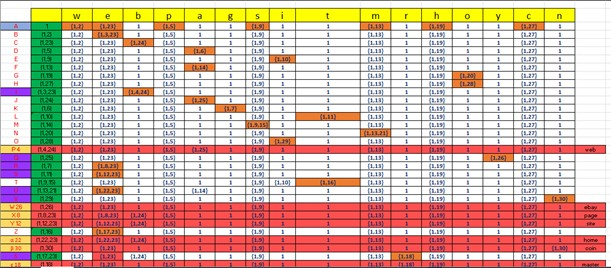
\includegraphics[height = 6cm]{tabla.jpg}		
	
	\section*{Capturas del Funcionamiento}
	En esta sección se encuentran las capturas de pantalla del funcionamiento del programa, tanto de la consola, como de los archivos generados.
	Las capturas se ordenaron comforme a la opción selecionada en el programa: 
	\begin{enumerate}
		\item \textbf{Lectura desde Archivo}
		\begin{itemize}
			\item 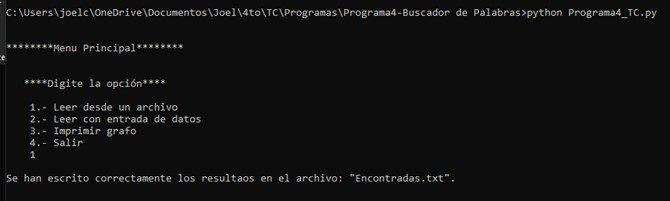
\includegraphics[height = 4cm]{LA1.jpg}
			\item 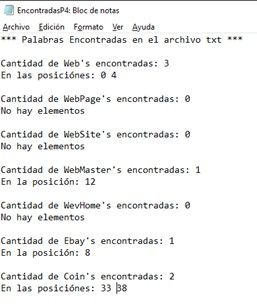
\includegraphics[height = 4cm]{LA2.jpg}
			\item 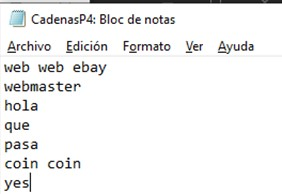
\includegraphics[height = 4cm]{L4.jpg}
			\item 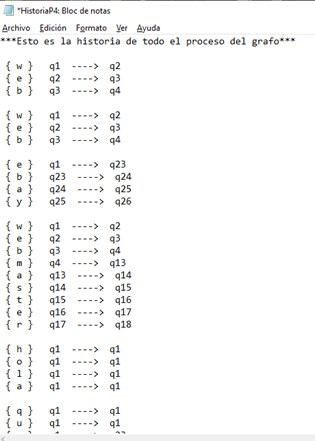
\includegraphics[height = 4cm]{LA3.jpg}os...
		\end{itemize}				
		\item \textbf{Lectura desde el teclado}
		\begin{itemize}
			\item 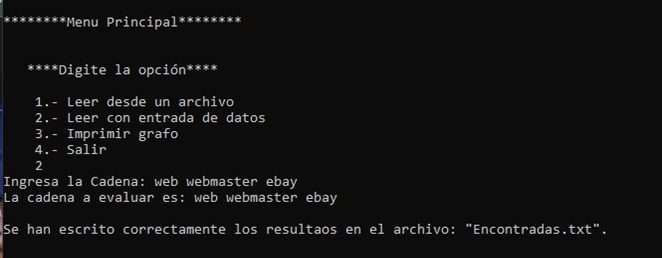
\includegraphics[height = 4cm]{LT1.jpg}
			\item 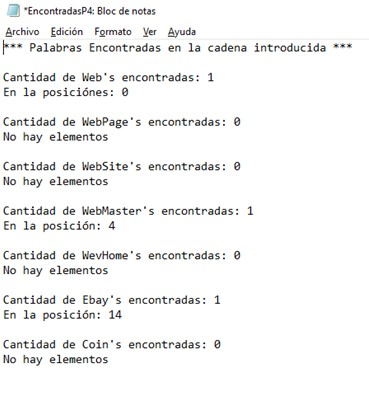
\includegraphics[height = 4cm]{LT4.jpg}os...
			\item 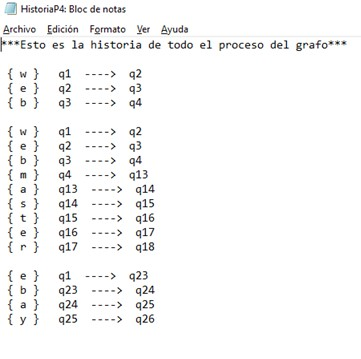
\includegraphics[height = 4cm]{LT3.jpg}
		\end{itemize}
		\item \textbf{Imprimir el Grafo}
		\begin{itemize}
			\item 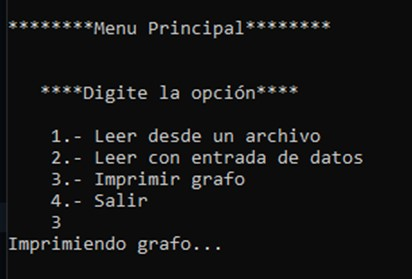
\includegraphics[height = 4cm]{IG1.jpg}
			\item 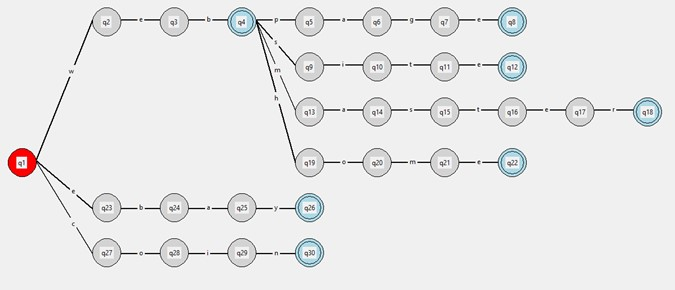
\includegraphics[height = 4cm]{IG2.jpg}
		\end{itemize}
		
	\end{enumerate}
	\section*{Código}
	\begin{python}
		#Programa 4.Buscador de Palabras
		# Nombre: Colin Ramiro Joel
		# Profesor: Juarez Martinez Genaro
		# Grupo: 4CM2
		# Materia: Teoria Computacional
		from tkinter import*
		def evaluacion(opcion):
			archivo = open("CadenasP4.txt", "r") 
			if opcion == 1:
				# archivo = open("Cadenas.txt", "r") 
				palabra = archivo.read()    
			elif opcion == 2:
				palabra = input("Ingresa la Cadena: ")    
			print("La cadena a evaluar es: " + palabra)    
			web = []
			webpage = [] 
			website = []
			webmaster = []
			webhome = []
			ebay = []
			coin = []     
			contAux = 0
			estado = 1
			sigEstado = estado    
			historia = open("HistoriaP4.txt","w")
			historia.write("***Esto es la historia de todo el proceso del grafo***\n\n")
			for letra in palabra:     				        
				if (estado == 1):          
					if (letra == "w"):                
						sigEstado = 2 
						historia.write(" { " + str(letra) + " } " + "  q" + str(estado) + "  ---->  q" + str(sigEstado) + "\n")
						estado = sigEstado           
					elif (letra == "e"):
						sigEstado = 23     
						historia.write(" { " + str(letra) + " } " + "  q" + str(estado) + "  ---->  q" + str(sigEstado) + "\n")
						estado = sigEstado  
					elif (letra == "c"):
						sigEstado = 27
						historia.write(" { " + str(letra) + " } " + "  q" + str(estado) + "  ---->  q" + str(sigEstado) + "\n")
						estado = sigEstado 
					else:
						sigEstado = 1
						historia.write(" { " + str(letra) + " } " + "  q" + str(estado) + "  ---->  q" + str(sigEstado) + "\n")
						estado = sigEstado                    
					continue         
			
				if (estado == 2):
					if (letra == "w"):
						sigEstado = 2
						historia.write(" { " + str(letra) + " } " + "  q" + str(estado) + "  ---->  q" + str(sigEstado) + "\n")
						estado = sigEstado
					elif (letra == "e"): 
						sigEstado = 3
						historia.write(" { " + str(letra) + " } " + "  q" + str(estado) + "  ---->  q" + str(sigEstado) + "\n")
						estado = sigEstado               
					else:
						sigEstado = 1
						historia.write(" { " + str(letra) + " } " + "  q" + str(estado) + "  ---->  q" + str(sigEstado) + "\n")
						estado = sigEstado
					continue
			
				if (estado == 3):
					if (letra == "w"):
						sigEstado = 2   
						historia.write(" { " + str(letra) + " } " + "  q" + str(estado) + "  ---->  q" + str(sigEstado) + "\n")
						estado = sigEstado                              
					elif (letra == "b"): 
						sigEstado = 4
						historia.write(" { " + str(letra) + " } " + "  q" + str(estado) + "  ---->  q" + str(sigEstado) + "\n")
						estado = sigEstado
						web.append(cont-3) #WEB         
					else:
						sigEstado = 1
						historia.write(" { " + str(letra) + " } " + "  q" + str(estado) + "  ---->  q" + str(sigEstado) + "\n")
						estado = sigEstado
					continue
			
				if (estado == 4): #FIN WEB
					if (letra == "w"):
						sigEstado = 2   
						historia.write(" { " + str(letra) + " } " + "  q" + str(estado) + "  ---->  q" + str(sigEstado) + "\n")
						estado = sigEstado               
					elif(letra == "p"):
						sigEstado = 5
						historia.write(" { " + str(letra) + " } " + "  q" + str(estado) + "  ---->  q" + str(sigEstado) + "\n")
						estado = sigEstado    
					elif(letra == "s"):
						sigEstado = 9
						historia.write(" { " + str(letra) + " } " + "  q" + str(estado) + "  ---->  q" + str(sigEstado) + "\n")
						estado = sigEstado    
					elif(letra == "m"):
						sigEstado = 13
						historia.write(" { " + str(letra) + " } " + "  q" + str(estado) + "  ---->  q" + str(sigEstado) + "\n")
						estado = sigEstado  
					elif(letra == "h"):
						sigEstado = 19
						historia.write(" { " + str(letra) + " } " + "  q" + str(estado) + "  ---->  q" + str(sigEstado) + "\n")
						estado = sigEstado    
					else:
						sigEstado = 1   
						historia.write("\n")
						estado = sigEstado
					continue
			
				if (estado == 5):   
					if (letra == "w"):
						sigEstado = 2   
						historia.write(" { " + str(letra) + " } " + "  q" + str(estado) + "  ---->  q" + str(sigEstado) + "\n")
						estado = sigEstado              
					elif(letra == "a"):
						sigEstado = 6
						historia.write(" { " + str(letra) + " } " + "  q" + str(estado) + "  ---->  q" + str(sigEstado) + "\n")
						estado = sigEstado            
					else:
						sigEstado = 1
						historia.write(" { " + str(letra) + " } " + "  q" + str(estado) + "  ---->  q" + str(sigEstado) + "\n")
						estado = sigEstado
					continue
			
				if (estado == 6):
					if (letra == "w"):
						sigEstado = 2   
						historia.write(" { " + str(letra) + " } " + "  q" + str(estado) + "  ---->  q" + str(sigEstado) + "\n")
						estado = sigEstado              
					elif(letra == "g"):
						sigEstado = 7
						historia.write(" { " + str(letra) + " } " + "  q" + str(estado) + "  ---->  q" + str(sigEstado) + "\n")
						estado = sigEstado            
					else:
						sigEstado = 1
						historia.write(" { " + str(letra) + " } " + "  q" + str(estado) + "  ---->  q" + str(sigEstado) + "\n")
						estado = sigEstado
					continue        
			
				if (estado == 7):            
					if (letra == "w"):
						sigEstado = 2   
						historia.write(" { " + str(letra) + " } " + "  q" + str(estado) + "  ---->  q" + str(sigEstado) + "\n")
						estado = sigEstado 
					elif (letra == "e"):
						sigEstado = 8
						historia.write(" { " + str(letra) + " } " + "  q" + str(estado) + "  ---->  q" + str(sigEstado) + "\n")
						estado = sigEstado
						webpage.append(cont-7) #WEBPAGE           
					else:
						sigEstado = 1
						historia.write(" { " + str(letra) + " } " + "  q" + str(estado) + "  ---->  q" + str(sigEstado) + "\n")
						estado = sigEstado
					continue
			
				if (estado == 8): #FIN WEBPAGE                   
					sigEstado = 1
					historia.write("\n")
					estado = sigEstado
				continue
			
				if (estado == 9):
					if (letra == "w"):
						sigEstado = 2
						historia.write(" { " + str(letra) + " } " + "  q" + str(estado) + "  ---->  q" + str(sigEstado) + "\n")
						estado = sigEstado              
					elif (letra == "i"):
						sigEstado = 10
						historia.write(" { " + str(letra) + " } " + "  q" + str(estado) + "  ---->  q" + str(sigEstado) + "\n")
						estado = sigEstado            
					else:
						sigEstado = 1
						historia.write(" { " + str(letra) + " } " + "  q" + str(estado) + "  ---->  q" + str(sigEstado) + "\n")
						estado = sigEstado
					continue
			
				if (estado == 10):
					if (letra == "w"):
						sigEstado = 2    
						historia.write(" { " + str(letra) + " } " + "  q" + str(estado) + "  ---->  q" + str(sigEstado) + "\n")
						estado = sigEstado       
					elif (letra == "t"):
						sigEstado = 11
						historia.write(" { " + str(letra) + " } " + "  q" + str(estado) + "  ---->  q" + str(sigEstado) + "\n")
						estado = sigEstado            
					else:
						sigEstado = 1
						historia.write(" { " + str(letra) + " } " + "  q" + str(estado) + "  ---->  q" + str(sigEstado) + "\n")
						estado = sigEstado
					continue
			
				if (estado == 11):
					if (letra == "w"):
						sigEstado = 2    
						historia.write(" { " + str(letra) + " } " + "  q" + str(estado) + "  ---->  q" + str(sigEstado) + "\n")
						estado = sigEstado       
					elif (letra == "e"):
						sigEstado = 12
						historia.write(" { " + str(letra) + " } " + "  q" + str(estado) + "  ---->  q" + str(sigEstado) + "\n")
						estado = sigEstado
						website.append(cont-7) #WEBSITE               
					else:
						sigEstado = 1     
						historia.write(" { " + str(letra) + " } " + "  q" + str(estado) + "  ---->  q" + str(sigEstado) + "\n")
						estado = sigEstado      
					continue
			
				if (estado == 12): #FIN WEBSITE
					sigEstado = 1
					historia.write("\n")
					estado = sigEstado
				continue
					
				if (estado == 13):
					if (letra == "w"):
						sigEstado = 2   
						historia.write(" { " + str(letra) + " } " + "  q" + str(estado) + "  ---->  q" + str(sigEstado) + "\n")
						estado = sigEstado            
					elif (letra == "a"):
						sigEstado = 14    
						historia.write(" { " + str(letra) + " } " + "  q" + str(estado) + "  ---->  q" + str(sigEstado) + "\n")
						estado = sigEstado         
					else:
						sigEstado = 1
						historia.write(" { " + str(letra) + " } " + "  q" + str(estado) + "  ---->  q" + str(sigEstado) + "\n")
						estado = sigEstado
					continue
			
				if (estado == 14):
					if (letra == "w"):
						sigEstado = 2  
						historia.write(" { " + str(letra) + " } " + "  q" + str(estado) + "  ---->  q" + str(sigEstado) + "\n")
						estado = sigEstado                     
					elif (letra == "s"): 
						sigEstado = 15    
						historia.write(" { " + str(letra) + " } " + "  q" + str(estado) + "  ---->  q" + str(sigEstado) + "\n")
						estado = sigEstado         
					else:
						sigEstado = 1
						historia.write(" { " + str(letra) + " } " + "  q" + str(estado) + "  ---->  q" + str(sigEstado) + "\n")
						estado = sigEstado
					continue
			
				if (estado == 15):
					if (letra == "w"):
						sigEstado = 2            
						historia.write(" { " + str(letra) + " } " + "  q" + str(estado) + "  ---->  q" + str(sigEstado) + "\n")
						estado = sigEstado           
					elif (letra == "t"):
						sigEstado = 16 
						historia.write(" { " + str(letra) + " } " + "  q" + str(estado) + "  ---->  q" + str(sigEstado) + "\n")
						estado = sigEstado                    
					else:
						sigEstado = 1
						historia.write(" { " + str(letra) + " } " + "  q" + str(estado) + "  ---->  q" + str(sigEstado) + "\n")
						estado = sigEstado
					continue
			
				if (estado == 16):
					if (letra == "w"):
						sigEstado = 2   
						historia.write(" { " + str(letra) + " } " + "  q" + str(estado) + "  ---->  q" + str(sigEstado) + "\n")
						estado = sigEstado        
					elif (letra == "e"):
						sigEstado = 17 
						historia.write(" { " + str(letra) + " } " + "  q" + str(estado) + "  ---->  q" + str(sigEstado) + "\n")
						estado = sigEstado           
					else:
						sigEstado = 1
						historia.write("\n")
						estado = sigEstado       
					continue
			
				if (estado == 17):
					if (letra == "w"):
						sigEstado = 2    
						historia.write(" { " + str(letra) + " } " + "  q" + str(estado) + "  ---->  q" + str(sigEstado) + "\n")
						estado = sigEstado     			
					elif (letra == "r"):
						sigEstado = 18
						historia.write(" { " + str(letra) + " } " + "  q" + str(estado) + "  ---->  q" + str(sigEstado) + "\n")
						estado = sigEstado
						webmaster.append(cont-9) #WEBMASTER
					elif (letra == "h"):
						sigEstado = 19
						historia.write(" { " + str(letra) + " } " + "  q" + str(estado) + "  ---->  q" + str(sigEstado) + "\n")
						estado = sigEstado
					elif (letra == "e"):
						sigEstado = 23    
						historia.write(" { " + str(letra) + " } " + "  q" + str(estado) + "  ---->  q" + str(sigEstado) + "\n")
						estado = sigEstado        
					elif (letra == "c"): 
						sigEstado = 27
						historia.write(" { " + str(letra) + " } " + "  q" + str(estado) + "  ---->  q" + str(sigEstado) + "\n")
						estado = sigEstado
					else:
						sigEstado = 1
						historia.write(" { " + str(letra) + " } " + "  q" + str(estado) + "  ---->  q" + str(sigEstado) + "\n")
						estado = sigEstado
					continue
			
				if (estado == 18): #FIN WEBMASTER
					sigEstado = 1
					historia.write("\n")
					estado = sigEstado
				continue
			
				if (estado == 19):
					if (letra == "w"):
						sigEstado = 2    
						historia.write(" { " + str(letra) + " } " + "  q" + str(estado) + "  ---->  q" + str(sigEstado) + "\n")
						estado = sigEstado
					elif (letra == "o"):
						sigEstado = 20
						historia.write(" { " + str(letra) + " } " + "  q" + str(estado) + "  ---->  q" + str(sigEstado) + "\n")
						estado = sigEstado            
					else:
						sigEstado = 1
						historia.write(" { " + str(letra) + " } " + "  q" + str(estado) + "  ---->  q" + str(sigEstado) + "\n")
						estado = sigEstado
					continue
			
				if (estado == 20):
					if (letra == "w"):
						sigEstado = 2 
						historia.write(" { " + str(letra) + " } " + "  q" + str(estado) + "  ---->  q" + str(sigEstado) + "\n")
						estado = sigEstado       
					elif (letra == "m"):
						sigEstado = 21
						historia.write(" { " + str(letra) + " } " + "  q" + str(estado) + "  ---->  q" + str(sigEstado) + "\n")
						estado = sigEstado            
					else:
						sigEstado = 1
						historia.write(" { " + str(letra) + " } " + "  q" + str(estado) + "  ---->  q" + str(sigEstado) + "\n")
						estado = sigEstado
					continue
			
				if (estado == 21):
					if (letra == "w"):
						sigEstado = 2       
						historia.write(" { " + str(letra) + " } " + "  q" + str(estado) + "  ---->  q" + str(sigEstado) + "\n")
						estado = sigEstado    
					elif (letra == "e"):
						sigEstado = 22
						historia.write(" { " + str(letra) + " } " + "  q" + str(estado) + "  ---->  q" + str(sigEstado) + "\n")
						estado = sigEstado
						webhome.append(cont-7) #WEBHOME            
					else:
						sigEstado = 1
						historia.write(" { " + str(letra) + " } " + "  q" + str(estado) + "  ---->  q" + str(sigEstado) + "\n")
						estado = sigEstado
					continue
			
				if (estado == 22): #FIN WEBHOME
					sigEstado = 1  
					historia.write("\n")
					estado = sigEstado
				continue
			
				if (estado == 23):             
					if (letra == "e"):
						sigEstado = 23
						historia.write(" { " + str(letra) + " } " + "  q" + str(estado) + "  ---->  q" + str(sigEstado) + "\n")
						estado = sigEstado
					elif (letra == "b"):
						sigEstado = 24    
						historia.write(" { " + str(letra) + " } " + "  q" + str(estado) + "  ---->  q" + str(sigEstado) + "\n")
						estado = sigEstado             
					else:
						sigEstado = 1
						historia.write(" { " + str(letra) + " } " + "  q" + str(estado) + "  ---->  q" + str(sigEstado) + "\n")
						estado = sigEstado
					continue
			
				if (estado == 24):             
					if (letra == "e"):
						sigEstado = 23
						historia.write(" { " + str(letra) + " } " + "  q" + str(estado) + "  ---->  q" + str(sigEstado) + "\n")
						estado = sigEstado            
					elif (letra == "a"):
						sigEstado = 25    
						historia.write(" { " + str(letra) + " } " + "  q" + str(estado) + "  ---->  q" + str(sigEstado) + "\n")
						estado = sigEstado                
					else:
						sigEstado = 1
						historia.write(" { " + str(letra) + " } " + "  q" + str(estado) + "  ---->  q" + str(sigEstado) + "\n")
						estado = sigEstado
					continue
			
				if (estado == 25):            
					if (letra == "e"):
						sigEstado = 23     
						historia.write(" { " + str(letra) + " } " + "  q" + str(estado) + "  ---->  q" + str(sigEstado) + "\n")
						estado = sigEstado            
					elif (letra == "y"):
						sigEstado = 26
						historia.write(" { " + str(letra) + " } " + "  q" + str(estado) + "  ---->  q" + str(sigEstado) + "\n")
						estado = sigEstado
						ebay.append(cont-4) #EBAY            
					else:
						sigEstado = 1
						historia.write(" { " + str(letra) + " } " + "  q" + str(estado) + "  ---->  q" + str(sigEstado) + "\n")
						estado = sigEstado
					continue        
			
				if (estado == 26): #FIN EBAY
					sigEstado = 1
					historia.write("\n")
					estado = sigEstado
				continue
			
				if (estado == 27):            
					if (letra == "c"):
						sigEstado = 27
						historia.write(" { " + str(letra) + " } " + "  q" + str(estado) + "  ---->  q" + str(sigEstado) + "\n")
						estado = sigEstado
					elif (letra == "o"):
						sigEstado = 28    
						historia.write(" { " + str(letra) + " } " + "  q" + str(estado) + "  ---->  q" + str(sigEstado) + "\n")
						estado = sigEstado         
					else:
						sigEstado = 1
						historia.write(" { " + str(letra) + " } " + "  q" + str(estado) + "  ---->  q" + str(sigEstado) + "\n")
						estado = sigEstado
					continue
			
				if (estado == 28):                  
					if (letra == "c"):
						sigEstado = 27
						historia.write(" { " + str(letra) + " } " + "  q" + str(estado) + "  ---->  q" + str(sigEstado) + "\n")
						estado = sigEstado              
					elif (letra == "i"):
						sigEstado = 29     
						historia.write(" { " + str(letra) + " } " + "  q" + str(estado) + "  ---->  q" + str(sigEstado) + "\n")
						estado = sigEstado        
					else:
						sigEstado = 1
						historia.write(" { " + str(letra) + " } " + "  q" + str(estado) + "  ---->  q" + str(sigEstado) + "\n")
						estado = sigEstado 
					continue
			
				if (estado == 29):                    
					if (letra == "c"):
						sigEstado = 27
						historia.write(" { " + str(letra) + " } " + "  q" + str(estado) + "  ---->  q" + str(sigEstado) + "\n")
						estado = sigEstado              
					elif (letra == "n"):
						sigEstado = 30
						historia.write(" { " + str(letra) + " } " + "  q" + str(estado) + "  ---->  q" + str(sigEstado) + "\n")
						estado = sigEstado 
						coin.append(cont-4) #COIN            
					else:
						sigEstado = 1
						historia.write(" { " + str(letra) + " } " + "  q" + str(estado) + "  ---->  q" + str(sigEstado) + "\n")
						estado = sigEstado 
					continue
			
				if (estado == 30): #FIN COIN
					sigEstado = 1
					historia.write("\n")
					estado = sigEstado 
				continue
				
				contAux = contAux + 1
			resultado = open("EncontradasP4.txt","w")
			if(opc == 1):
				resultado.write("*** Palabras Encontradas en el archivo txt ***\n\n")
			elif(opc == 2):
				resultado.write("*** Palabras Encontradas en la cadena introducida ***\n\n")
			#Palabra web    
			resultado.write("Cantidad de Web's encontradas: ")
			resultado.write(str(len(web)) + "\n")
			if(str(len(web)) == "0"):
				resultado.write("No hay elementos.")
			elif(str(len(web)) == "1"):
				resultado.write("En la posicion: ")
				resultado.write(" ")  
			else:  
				resultado.write("En las posiciones: ")
				resultado.write(" ")  
			for elementos in web:
				resultado.write(str(elementos) + " ")
			resultado.write("\n\n")
			
			#Palabra webpage    
			resultado.write("Cantidad de WebPage's encontradas: ")
			resultado.write(str(len(webpage)) + "\n")
			if(str(len(webpage)) == "0"):
				resultado.write("No hay elementos")
			elif(str(len(webpage)) == "1"):
				resultado.write("En la posicion: ")
				resultado.write(" ") 
				for elementos in webpage:
					resultado.write(str(elementos) + " ") 
			else:  
				resultado.write("En las posiciones: ")
				resultado.write(" ") 
			for elementos in webpage:
				resultado.write(str(elementos) + " ")     
			resultado.write("\n\n")
			
			#Palabra website    
			resultado.write("Cantidad de WebSite's encontradas: ")
			resultado.write(str(len(website)) + "\n")
			if(str(len(website)) == "0"):
				resultado.write("No hay elementos")
			elif(str(len(website)) == "1"):
				resultado.write("En la posicion: ")
				resultado.write(" ") 
				for elementos in website:
					resultado.write(str(elementos) + " ") 
			else:  
				resultado.write("En las posiciones: ")
				resultado.write(" ") 
				for elementos in website:
					resultado.write(str(elementos) + " ")     
			resultado.write("\n\n")
			
			#Palabra webmaster    
			resultado.write("Cantidad de WebMaster's encontradas: ")
			resultado.write(str(len(webmaster)) + "\n")
			if(str(len(webmaster)) == "0"):
				resultado.write("No hay elementos")
			elif(str(len(webmaster)) == "1"):
				resultado.write("En la posicion: ")
				resultado.write(" ") 
				for elementos in webmaster:
					resultado.write(str(elementos) + " ") 
			else:  
				resultado.write("En las posiciones: ")
				resultado.write(" ") 
				for elementos in webmaster:
					resultado.write(str(elementos) + " ")     
			resultado.write("\n\n")
			
			#Palabra webhome
			resultado.write("Cantidad de WevHome's encontradas: ")
			resultado.write(str(len(webhome)) + "\n")
			if(str(len(webhome)) == "0"):
				resultado.write("No hay elementos")
			elif(str(len(webhome)) == "1"):
				resultado.write("En la posicion: ")
				resultado.write(" ") 
				for elementos in webhome:
					resultado.write(str(elementos) + " ") 
			else:  
				resultado.write("En las posiciones: ")
				resultado.write(" ") 
				for elementos in webhome:
					resultado.write(str(elementos) + " ")     
			resultado.write("\n\n")
		
			#Palabra ebay
			resultado.write("Cantidad de Ebay's encontradas: ")
			resultado.write(str(len(ebay)) + "\n")
			if(str(len(ebay)) == "0"):
				resultado.write("No hay elementos")
			elif(str(len(ebay)) == "1"):
				resultado.write("En la posicion: ")
				resultado.write(" ") 
				for elementos in ebay:
					resultado.write(str(elementos) + " ") 
			else:  
				resultado.write("En las posiciones: ")
				resultado.write(" ") 
				for elementos in ebay:
					resultado.write(str(elementos) + " ")     
			resultado.write("\n\n")
			
			#Palabra coin
			resultado.write("Cantidad de Coin's encontradas: ")
			resultado.write(str(len(coin)) + "\n")
			if(str(len(coin)) == "0"):
				resultado.write("No hay elementos")
			elif(str(len(coin)) == 1):
				resultado.write("En la posicion: ")
				resultado.write(" ") 
				for elementos in coin:
					resultado.write(str(elementos) + " ") 
			else:  
				resultado.write("En las posiciones: ")
				resultado.write(" ") 
				for elementos in coin:
					resultado.write(str(elementos) + " ")     
			resultado.write("\n\n")    
			print("\nSe han escrito correctamente los resultados en el archivo: \"Encontradas.txt\".")    
			resultado.close()
			archivo.close()
			
		def ilustrarGrafo(): #Funcion que muestra el grafo
			ventana = Tk()
			vent = Canvas(ventana,width=2000,height=2000)
			ventana.geometry("2000x2000")
			ventana.title("Grafo")
			#LINEAS    
			vent.create_line(100, 330, 200, 82, width=2, fill='black') #WEB
			vent.create_line(230, 82, 920, 82, width=2, fill='black') #WEBPAGE
			vent.create_line(490, 82, 560, 162, width=2, fill='black') #WEBSITE
			vent.create_line(560, 162, 920, 162, width=2, fill='black') #WEBSITE
			vent.create_line(490, 82, 560, 242, width=2, fill='black') #WEBMASTER
			vent.create_line(560, 242, 1160, 242, width=2, fill='black') #WEBMASTER
			vent.create_line(490, 82, 560, 335, width=2, fill='black') #WEBHOME
			vent.create_line(560, 335, 920, 335, width=2, fill='black') #WEBHOME 
			vent.create_line(98, 330, 200, 417, width=2, fill='black') #EBAY
			vent.create_line(230, 417, 560, 417, width=2, fill='black') #EBAY
			vent.create_line(98, 330, 200, 497, width=2, fill='black') #COIN
			vent.create_line(230, 497, 560, 497, width=2, fill='black') #COIN  
			#NODOS    
			vent.create_oval(50,310,100,360, fill="red")#Q1 Inicial
			q1 = Label(ventana,text="q1").place(x=65,y=325)
			#WEB
			vent.create_oval(200,60,250,110, fill="light gray") #Q2
			q2 = Label(ventana,text="q2").place(x=215,y=75)
			w1 = Label(ventana,text="w").place(x=155,y=162)
			vent.create_oval(320,60,370,110, fill="light gray") #Q3
			q3 = Label(ventana,text="q3").place(x=335,y=75)   
			e1 = Label(ventana,text="e").place(x=280,y=70) 
			vent.create_oval(440,60,490,110, fill="light blue") #Q4
			vent.create_oval(445,65,485,105, fill="light blue") #Q4 Final
			q4 = Label(ventana,text="q4").place(x=455,y=75)   
			b1 = Label(ventana,text="b").place(x=400,y=70) 
			#WEBPAGE
			vent.create_oval(560,60,610,110, fill="light gray") #Q5
			q5 = Label(ventana,text="q5").place(x=575,y=75)
			p1 = Label(ventana,text="p").place(x=520,y=70)
			vent.create_oval(680,60,730,110, fill="light gray") #Q6
			q6 = Label(ventana,text="q6").place(x=695,y=75)
			a1 = Label(ventana,text="a").place(x=640,y=70)
			vent.create_oval(800,60,850,110, fill="light gray") #Q7
			q7 = Label(ventana,text="q7").place(x=815,y=75)
			g1 = Label(ventana,text="g").place(x=760,y=70)
			vent.create_oval(920,60,970,110, fill="light blue") #Q8 
			vent.create_oval(925,65,965,105, fill="light blue") #Q8 Final
			q8 = Label(ventana,text="q8").place(x=935,y=75)
			e2 = Label(ventana,text="e").place(x=880,y=70)    
			#WEBSITE
			vent.create_oval(560,140,610,190, fill="light gray") #Q9
			q9 = Label(ventana,text="q9").place(x=575,y=155)
			s1 = Label(ventana,text="s").place(x=520,y=110)
			vent.create_oval(680,140,730,190, fill="light gray") #Q10
			q10 = Label(ventana,text="q10").place(x=693,y=155)
			i1 = Label(ventana,text="i").place(x=640,y=150)
			vent.create_oval(800,140,850,190, fill="light gray") #Q11
			q11 = Label(ventana,text="q11").place(x=813,y=155)
			t1 = Label(ventana,text="t").place(x=760,y=150)
			vent.create_oval(920,140,970,190, fill="light blue") #Q12
			vent.create_oval(925,145,965,185, fill="light blue") #Q12
			q12 = Label(ventana,text="q12").place(x=933,y=155)
			e3 = Label(ventana,text="e").place(x=880,y=150)
			#WEBMASTER
			vent.create_oval(560,220,610,270, fill="light gray") #Q13
			q13 = Label(ventana,text="q13").place(x=573,y=235)
			m1 = Label(ventana,text="m").place(x=520,y=160)
			vent.create_oval(680,220,730,270, fill="light gray") #Q14
			q14 = Label(ventana,text="q14").place(x=693,y=235)
			a2 = Label(ventana,text="a").place(x=640,y=230)
			vent.create_oval(800,220,850,270, fill="light gray") #Q15
			q15 = Label(ventana,text="q15").place(x=813,y=235)
			s2 = Label(ventana,text="s").place(x=760,y=230)
			vent.create_oval(920,220,970,270, fill="light gray") #Q16
			q16 = Label(ventana,text="q16").place(x=933,y=235)
			t2 = Label(ventana,text="t").place(x=880,y=230)
			vent.create_oval(1040,220,1090,270, fill="light gray") #Q17
			q17 = Label(ventana,text="q17").place(x=1053,y=235)
			e4 = Label(ventana,text="e").place(x=1000,y=230)
			vent.create_oval(1160,220,1210,270, fill="light blue") #Q18
			vent.create_oval(1165,225,1205,265, fill="light blue") #Q18
			q18 = Label(ventana,text="q18").place(x=1173,y=235)
			r1 = Label(ventana,text="r").place(x=1120,y=230)
			#WEBHOME
			vent.create_oval(560,310,610,360, fill="light gray") #Q19
			q19 = Label(ventana,text="q19").place(x=573,y=325)
			h1 = Label(ventana,text="h").place(x=520,y=210)
			vent.create_oval(680,310,730,360, fill="light gray") #Q20
			q20 = Label(ventana,text="q20").place(x=693,y=325)
			o1 = Label(ventana,text="o").place(x=640,y=323)
			vent.create_oval(800,310,850,360, fill="light gray") #Q21
			q21 = Label(ventana,text="q21").place(x=813,y=325)
			m2 = Label(ventana,text="m").place(x=760,y=323)
			vent.create_oval(920,310,970,360, fill="light blue") #Q22
			vent.create_oval(925,315,965,355, fill="light blue") #Q22
			q22 = Label(ventana,text="q22").place(x=933,y=325)
			e5 = Label(ventana,text="e").place(x=880,y=323)
			#EBAY
			vent.create_oval(200,390,250,440, fill="light gray") #Q19
			q23 = Label(ventana,text="q23").place(x=213,y=405)
			e6 = Label(ventana,text="e").place(x=160,y=375)
			vent.create_oval(320,390,370,440, fill="light gray") #Q20
			q24 = Label(ventana,text="q24").place(x=333,y=405)
			b1 = Label(ventana,text="b").place(x=280,y=404)
			vent.create_oval(440,390,490,440, fill="light gray") #Q21
			q25 = Label(ventana,text="q25").place(x=453,y=405)
			a3 = Label(ventana,text="a").place(x=400,y=404)
			vent.create_oval(560,390,610,440, fill="light blue") #Q22
			vent.create_oval(565,395,605,435, fill="light blue") #Q22
			q26 = Label(ventana,text="q26").place(x=573,y=405)
			y1 = Label(ventana,text="y").place(x=520,y=404)   
			#COIN
			vent.create_oval(200,470,250,520, fill="light gray") #Q23
			q27 = Label(ventana,text="q27").place(x=213,y=485)
			c1 = Label(ventana,text="c").place(x=160,y=433)
			vent.create_oval(320,470,370,520, fill="light gray") #Q24
			q28 = Label(ventana,text="q28").place(x=333,y=485)
			o2 = Label(ventana,text="o").place(x=280,y=485)
			vent.create_oval(440,470,490,520, fill="light gray") #Q25
			q29 = Label(ventana,text="q29").place(x=453,y=485)
			i2 = Label(ventana,text="i").place(x=400,y=485)
			vent.create_oval(560,470,610,520, fill="light blue") #Q26
			vent.create_oval(565,475,605,515, fill="light blue") #Q26
			q30 = Label(ventana,text="q30").place(x=573,y=485)
			n1 = Label(ventana,text="n").place(x=520,y=485)        
			vent.place(x=0,y=0)
			ventana.mainloop()	
		opc = 0
		salir = 4
		while opc != salir:
		print("Menu Principal")
		print("Digite la opcion")
		opc = int(input('''
			1.- Leer desde un archivo
			2.- Leer con entrada de datos
			3.- Imprimir grafo
			4.- Salir
			'''))    
		if (opc == 1) or (opc == 2):
			evaluacion(opc)    
			elif opc == 3:
		print("Imprimiendo grafo...")
			ilustrarGrafo()
		elif opc == 4:
			print("Saliendo del Programa. Hasta Luego!!!!")
		else:
			print("Opcion invalida, Vuelva a intentar")
	\end{python}
	
	\section*{Conclusiones}
	Al término de la realización de esta práctica, pude reforzar los conocimientos que adquirí en clase. Se pudo concluir de manera correcta esta práctica junto con la ilustración del grafo mismo.
	
	Quiero añadir que fue sencillo de implementarse el programa en general ya que solo fue realizar un análisis profundo del autómata y más que nada los estados, asi como sus transiciones y cambios de estado a estado. Ya con este análisis únicamente fue transcribirlo a un código en Python para su ejecución.
	
	\section*{Referencias}
	\begin{enumerate}
		\item INAOE. (2017). Autómatas Finitos. Diciembre 21,2021, de INAOE Sitio web: https://ccc.inaoep.mx/~emorales/Cursos/Automatas/AutomatasFinitos.pdf
		\item JavaTpoint. (2011). NFA (Non-Deterministic finite automata). Diciembre 21,2021, de javaTpoint Sitio web: https://www.javatpoint.com/non-deterministic-finite-automata
		\item Universidad Nacional de Córdoba. (2015). Autómatas Finitos No-Deterministicos (NFA). Diciembre 21,2021, de Universidad Nacional de Córdoba Sitio web: https://wiki.cs.famaf.unc.edu.ar/lib/exe/fetch.php?media=intrologica:2015:class-2-handout-2015.pdf		
	\end{enumerate}
	
\end{document}